\documentclass[8pt]{beamer}
% Add references to notes
\makeatletter\defbeameroption{show only notes}[]{\beamer@notestrue\beamer@notesnormalsfalse}

% Originally from https://kbroman.org/blog/2013/10/07/better-looking-latexbeamer-slides/
\usetheme{default}
\hypersetup{pdfpagemode=UseNone} % hides bookmarks on initial view
\beamertemplatenavigationsymbolsempty % removes navigation buttons clashing with the defined slide numbers

\setbeamertemplate{sections/subsections in toc}[sections numbered] % replaces bullets in toc with numbers
\setbeamertemplate{bibliography item}{\insertbiblabel} % Numbered bibliography
\setbeamertemplate{itemize subitem}{{\textendash}} % changes bullets to \textendash
% Make bullets/nums smaller
\setbeamerfont{itemize/enumerate subbody}{size=\footnotesize}
\setbeamerfont{itemize/enumerate subitem}{size=\footnotesize}
% Slide number
 \setbeamertemplate{footline}{%
   \raisebox{5pt}{\makebox[\paperwidth]{\hfill\makebox[20pt]{\color{gray}
         \scriptsize\insertframenumber}}}\hspace*{5pt}}

\definecolor{foreground}{RGB}{255,255,255}
\definecolor{background}{RGB}{24,24,24}
\definecolor{title}{RGB}{107,174,214}
\definecolor{gray}{RGB}{155,155,155}
\definecolor{subtitle}{RGB}{102,255,204}
\definecolor{hilight}{RGB}{102,255,204}
\definecolor{vhilight}{RGB}{255,111,207}

\setbeamercolor{titlelike}{fg=title}
\setbeamercolor{subtitle}{fg=subtitle}
\setbeamercolor{institute}{fg=gray}
\setbeamercolor{normal text}{fg=foreground,bg=background}
\setbeamercolor{item}{fg=foreground} % color of bullets
\setbeamercolor{subitem}{fg=gray}
\setbeamercolor{itemize/enumerate subbody}{fg=gray}
\setbeamercolor{section in toc}{fg=foreground}
\setbeamercolor{subsection in toc}{fg=gray}


\usepackage{amsmath} % for more symbols and mafs
\usepackage{hyperref} % for links
\usepackage{fancyvrb}
\usepackage{hyperref}

\usepackage{array}
\newcolumntype{M}{>{\centering\arraybackslash}m{2.2cm}}
\newcolumntype{R}{>{\centering\arraybackslash}m{1.5cm}}

\usepackage{caption}
\captionsetup{justification=raggedleft} % right aligns multiline captions

\graphicspath{{../images/}}

\usepackage[backend=biber, sorting=none]{biblatex}
\addbibresource{../bib.bib}

\usepackage{xepersian} % must be the last package
\settextfont{XB Roya}
\setlatintextfont{Vazir}
\setdigitfont{XB Roya}
\setmonofont{Iosevka}
\usefonttheme{serif} % (Required for Persian)

\makeatletter
% Originally from http://qa.parsilatex.com/14100
% -----
% BEGIN List fix
% -----
\expandafter\let\csname beamer@@tmpop@itemize item@default\endcsname\relax
\expandafter\let\csname beamer@@tmpop@itemize subitem@default\endcsname\relax
\expandafter\let\csname beamer@@tmpop@itemize subsubitem@default\endcsname\relax

\defbeamertemplate*{itemize item}{default}{\scriptsize\raise1.25pt\hbox{\donotcoloroutermaths$\blacktriangleleft$}}
\defbeamertemplate*{itemize subitem}{default}{\tiny\raise1.5pt\hbox{\donotcoloroutermaths$\blacktriangleleft$}}
\defbeamertemplate*{itemize subsubitem}{default}{\tiny\raise1.5pt\hbox{\donotcoloroutermaths$\blacktriangleleft$}}

\patchcmd{\@listi}{\leftmargin}{\rightmargin}{}{}
\let\@listI\@listi
\patchcmd{\@listii}{\leftmargin}{\rightmargin}{}{}
\patchcmd{\@listiii}{\leftmargin}{\rightmargin}{}{}
\patchcmd{\beamer@enum@}{\raggedright}{\raggedleft}{}{}
\patchcmd{\@@description}{\raggedright}{\raggedleft}{}{}
\patchcmd{\@@description}{\leftmargin}{\rightmargin}{}{}

\renewcommand{\itemize}[1][]{
  \beamer@ifempty{#1}{}{\def\beamer@defaultospec{#1}}
  \ifnum \@itemdepth >2\relax\@toodeep\else
    \advance\@itemdepth\@ne
    \beamer@computepref\@itemdepth% sets \beameritemnestingprefix
    \usebeamerfont{itemize/enumerate \beameritemnestingprefix body}%
    \usebeamercolor[fg]{itemize/enumerate \beameritemnestingprefix body}%
    \usebeamertemplate{itemize/enumerate \beameritemnestingprefix body begin}%
    \list{\usebeamertemplate{itemize \beameritemnestingprefix item}}{\def\makelabel##1{{
      \hss\llap{{
        \usebeamerfont*{itemize \beameritemnestingprefix item}
        \usebeamercolor[fg]{itemize \beameritemnestingprefix item}##1}}
      }}
    }
  \fi
  \beamer@cramped
  \raggedleft
  \beamer@firstlineitemizeunskip
}
% -----
% END List fix
% -----
% BEGIN TOC fix
% -----
\expandafter\let\csname beamer@@tmpop@subsection in toc@default\endcsname\relax
\expandafter\let\csname beamer@@tmpop@subsubsection in toc@default\endcsname\relax
\defbeamertemplate*{subsection in toc}{default}
{\leavevmode\rightskip=1.5em\inserttocsubsection\par}

\defbeamertemplate*{subsubsection in toc}{default}
{\leavevmode\normalsize\usebeamerfont{subsection in toc}\rightskip=3em
  \usebeamerfont{subsubsection in toc}\inserttocsubsubsection\par}
% -----
% END TOC fix
% -----
\makeatother

\raggedleft % right aligns for Persian texts


\author{محمدیاسین داوده}
\title{لینوکس}
\subtitle{هرآنچه لازم است بدانید}
\date{\today}

\newcommand{\start}[1][نقشه راه]{
  \frame{\maketitle}
  \begin{frame}{#1}\tableofcontents\end{frame}
}

\newcommand{\bib}{
  \begin{LTR}
    \printbibliography[heading=none]
  \end{LTR}
}

\newcommand{\refs}{
  \section{مراجع}
  \begin{frame}[allowframebreaks]{مراجع}
    \bib
  \end{frame}
  \note{\bib}
}

\newcommand{\subt}[1]{{\footnotesize\color{subtitle}{#1}}}

\newcommand{\divider}[1]{\frame{\Huge{#1}}}

\newcommand{\subdivider}[1]{\frame{\color{hilight}\huge{#1}}}

\newcommand{\alongside}{\and\\\small\smallskip}

\newcommand{\singleton}[2][]{
  \begin{frame}{#1}
    \centering
    #2
  \end{frame}
}

\newcommand{\includetwins}[3][\textwidth]{
  \includegraphics[width=.49#1]{#2}
  \includegraphics[width=.49#1]{#3}
}
% -----
% BEGIN Code (minted)
% -----
\newenvironment{code*}[2][]{
  \VerbatimEnvironment
  \begin{LTR}
    \begin{minted}[#1, linenos, mathescape]{#2}%
    }{
    \end{minted}
  \end{LTR}
}

\newcommand{\codecaption}[1][]{\captionsetup{type=listings}\captionof{listing}{#1}}

\AtBeginEnvironment{minted}{\renewcommand{\fcolorbox}[4][]{#4}} % Disable syntax error red boxes
% -----
% END Code (minted)
% -----


\subtitle{قسمت دوم: نصب}
\author{مهدی صفریان \alongside محمدیاسین داوده}
\begin{document}
\start

% فارسی
\begin{frame}{نصب و راه‌اندازی دبین~\cite{deb_book}}
  دبین از قدیمی‌ترین توزیع‌هاست و با چند نصاب همراه است.
  \vfill
  \textbf{سیستم مورد نیاز برای نصب:}
  \begin{itemize}
    \item مینیمال بدون رابط گرافیکی:
    \begin{itemize}
      \item ۱۲۸ مگابایت رم
      \item ۲ گیگابایت حافظه
    \end{itemize}
    \item با پکیج‌های اضافی و رابطی رایج:
    \begin{itemize}
      \item ۱ گیگابایت رم
      \item ۱۰ گیگابایت حافظه
    \end{itemize}
  \end{itemize}
\end{frame}
\note{تلفظ: دِب-یَن (/\lr{\texttt{ˈdɛbiən}}/)}
\section{شروع نصب}
\divider{شروع نصب}
\begin{frame}{روش‌های مختلف نصب}
  راه‌های بوت فایل نصب:
  \begin{enumerate}
    \item دیسک
    \item حافظه جانبی
    \item شبکه
  \end{enumerate}
\end{frame}
\note{
  هرکدام انتخاب می‌شود که BIOS از آن پشتیبانی می‌کند. بایوس نرم‌افزاری در مادربرد است و زمان روش شدن سیستم اجرا می‌شود، تا کارهای پایه‌ای مانند راه‌اندازی سیستم‌عامل را انجام دهد.

  خیلی از BIOS‌ها این اجازه را می‌دهند که مراحل بوت شدن مستقیما با دانلود هسته و یک ایمیج خیلی کوچک از فایل سیستم‌ از طریق شبکه صورت گیرد.
  این متد نام‌های مختلفی دارد (مثلاً PXE یا بوت TFTP). هنگامی که دسترسی به CD-ROM یا درگاه USB ندارید شاید تنها راه باشد.

  در این متد مراحل نصب به دو قسمت تقسیم می‌شود.
  اول، زمانی که رایانه در حال بوت شدن است بایوس (یا کارت شبکه) به طور خودکار درخواست یک آدرس آی‌پی می‌دهد.
  بعد از اینکه سرور DHCP و BOOTP پاسخی دادند، پاسخ شامل filename و همچنین تنظیمات شبکه است.
  بعد از تنظیمات شبکه، کامپیوتر کاربر برای یک فایل که نامش در درخواست قبلی بود (filename) درخواست \lr{(Trivial File Transfer Protocol) TFTP} ارسال می‌کند.
  به محض رسیدن فایل، اجرا می‌شود و سپس برنامه نصاب دبین اجرا می‌شود و مراحل همانند دیگر حالات (مثلاً دیسک) ادامه می‌یابد.
}
\begin{frame}{انواع ایمیج}
  دبین دو ایمیج مینیمال و عادی دارد. مینمال سبک‌تر است و اگر نیاز باشد پکیج‌ها را از اینترنت دانلود می‌کند.
  \pic[.4]{debian-logo}{بخار برخاسته از جادوی دبین (لوگوی دبین)~\cite{fig:wp:deb}}
\end{frame}
\note{
  شما همچنین می‌توانید نصاب و ایمیج خود را بسازید و با آن نصب کنید.

  در نصب‌های مقایس بالا از نصاب‌های تمام اتوماتیک یا \lr{FAI (Fully Automatic Installer)} استفاده می‌کنند.
}
\begin{frame}{شروع نصب}
  هنگام بوت ایمیج یک بوت‌لودر باز می‌شود که به شما امکان تنظیم پارامترهای مختلف نصاب و شروع نصب را می‌دهد.
  \pic[.6]{bootloader}{صفحه بوت‌لودر اولیه~\cite{fig:deb:bootscreen}}
\end{frame}
\note{
  تفاوت ۳۲ بیتی و ۶۴ بیتی: فرق اصلی این دو معماری در سایز مموری است. از لحاظ نظری معماری ۳۲ بیتی نمی‌تواند با بیشتر از ۴ گیگ رم کار کند.

  مولتی بوت: اگر در سیستم حاضر ویندوز یا هر سیستم‌عامل دیگری نصب است لازم به حذف آن نیست و امکان استفاده هر دوی آنها در یک دیسک وجود دارد و فقط لازم است دیسک را با توجه به نیاز هر کدام از سیستم عامل‌ها پارتیشن‌بندی کرد، و در موقع بوت شدن رایانه هر کدام را که خواستید انتخاب کنید.

  به این نوع پیکربندی اصطلاحاً «Dual boot» یا «Multi boot» می‌گویند.

  بوت-لودر: یک برنامه سطح پایین است پس از بوت شدن رایانه توسط BIOS، بوت-لودر کرنل لینوکس را بارگذاری می‌کند.
  این نرم‌افزار معمولا یک منو دارد که به کاربر اجازه می‌دهد کرنل‌هایی بر روی رایانه نصب هستند را اجرا کند یا حتی سیستم عامل دیگری را اجرا کند. از معروف‌ترین بوت‌لودرها گراب (GRUB) است.
}
\begin{frame}{انتخاب زبان}
  \begin{figure}
    \includetwins{lang}{lang-cli}
    \caption*{مرحله انتخاب زبان نصاب در CLI و GUI از اولین مراحل نصب است.~\cite{fig:deb:lang_gui}}
  \end{figure}
\end{frame}
\begin{frame}{انتخاب کشور}
  در این مرحله موقعیت زمانی و مکانی در سیستم شما تنظیم می‌شود.
  \begin{figure}
    \includetwins{country-gui}{country-cli}
    \caption*{انتخاب کشور در محیط گرافیکی و متنی~\cite{fig:deb:country_gui}}
  \end{figure}
\end{frame}
\note{
  بعد از این مرحله بوت شدن کامل ایمیج، تمام فایل‌های لازم برای ادامه کار توسط نصاب بارگذاری می‌شود که شامل درایورهای اضافه برای باقی سخت افزارها است به خصوص کارت شبکه و دیگر سخت افزارهایی که در مراحل نصب دخیل هستند.

  پس از شناسایی شخت افزارها، نصاب به دنبال شناسایی کارت شبکه می‌رود و اگر در بارگذاری ماژول کارت شبکه شکست بخورد می‌توانید به صورت دستی ماژول را بارگذاری کنید.

  این مرحله باید کاملا تکمیل شود تا دیگر مراحل نصب نیز انجام شود چرا که خیلی از پکیج‌های دبین از طریق شبکه دانلود می‌شود.
}
\begin{frame}{تعیین رمز عبور کاربر root}
  کاربر روت مدیر اصلی سیستم و بالاترین سطح دسترسی است.
  \pic[.7]{sudo}{درخواست پسورد برای کاربر root~\cite{fig:deb:user_root}}
\end{frame}
\note{
  حساب کاربری «super-user» یا همان «sudo» مدیر اصلی سیستم شما است و قادر است تا بدون اینکه جلوی درخواستش گرفته شود هر دستوری را اجرا کند. به همین دلیل ممکن است خطرناک باشد اگر به درستی ندانید که چه کاری می‌کنید. کاربر روت یک سوپریوزر است.

  این کاربر هنگار نصب به طور خودکار ایجاد می‌شود و در این مرحله از شما درخواست رمز عبور می‌کند و برای تأیید آن یکبار دیگر نیز در همین مرحله از شما رمز را می‌پرسد.
 
  رمز عبور کاربر root ترجیحاً باید ۱۲ کارکتر یا بیشتر و ترکیبی از حروف و عدد باشد چرا که در سیستم‌های سروری که مورد حمله قرار می‌گیرندمعمولاً از دیکشنری رمز عبور استفاده می‌شود و به همین خاطر باید امنیت کافی را داشته باشد.

  اگر می‌خواهید کاربر root غیر فعال باشد آن دو فیلد را خالی بگذارید تا در مرحله بعد یک کاربر معمولی بسازید تا آن کاربر از حقوق کاربر root برخوردار باشد.
}
\begin{frame}{ساخت اولین کاربر}
  \pic[.8]{user-stn}{ساخت کاربر استاندارد~\cite{fig:deb:user_stn}}
\end{frame}
\singleton[شناسایی دیسک حافظه و دیگر سخت افزارها]{
  ساعت ابتدا بر اساس ساعت BIOS و سپس بر اساس NTP شبکه به طور خودکار تنظیم می‌شود.

  مرحله بعد آن شناسایی دیسک حافظه و باقی سخت افزارهاست که صورت خودکار صورت می گیرد.
}
\section{پارتیشن‌بندی}
\divider{پارتیشن‌بندی}
\begin{frame}{پارتیشن‌بندی}
  \textbf{دقت کنید! پارتیشن‌بندی می‌تواند به اطلاعات شما آسیب برساند!}
  نصاب دبین برای پارتیشن بندی ۴ روش ارائه می‌کند:
  \begin{itemize}
    \item استفاده از تمام دیسک
    \item استفاده از تمام دیسک و راه اندازی LVM
    \item استفاده از تمام دیسک و راه اندازی LVM رمزنگاری شده
    \item نصب دستی
  \end{itemize}
\end{frame}
\note{
  پارتیشن‌بندی معمولاً به عنوان سخت‌ترین مرحلهٔ نصب هر سیستم‌عاملی شناخته می‌شود.

  بجز نصب دستی تمام اطلاعات دیسک انتخاب شده پاک می‌شود. بهترین روش برای یادگیری و دقیقترین معمولاً نصب دستی است.

  % فارسی
  % TODO LVM
  LVM (Logical Volume Manager)
  نرم‌افزاری که به کرنل اجازهٔ نقشه سازی منطقی و مجازی سازی درایو را می‌دهد.
}

\begin{frame}{پارتیشن بندی}
  \begin{figure}
    \begin{columns}
      \column{0.5\textwidth}
      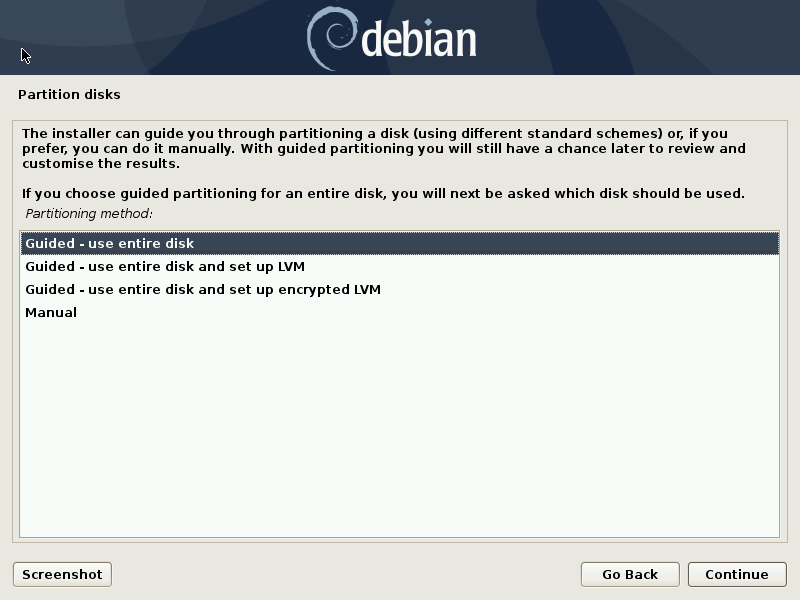
\includegraphics[scale=0.20]{partitioning}
      \caption*{انتخاب روش پارتیشن‌بندی~\cite{fig:deb:partitioning}}
      \column{0.5\textwidth}
      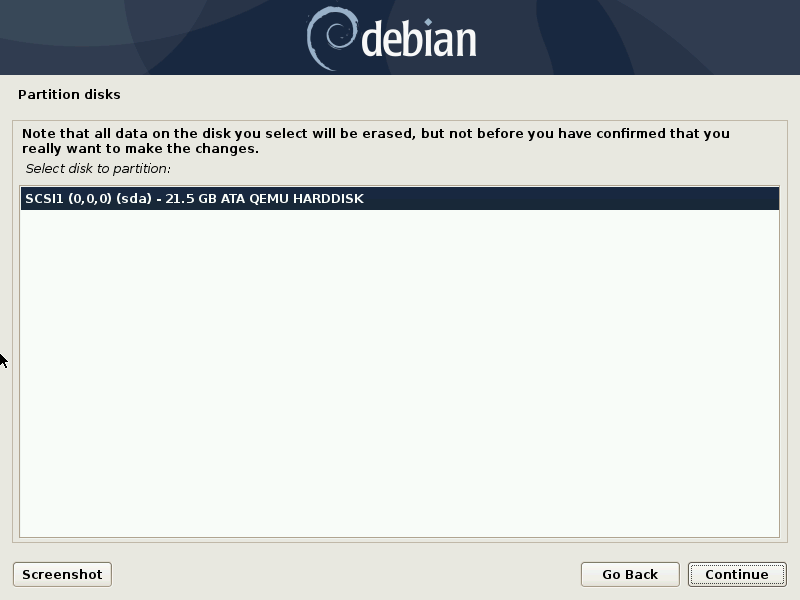
\includegraphics[scale=0.20]{disk}
      \caption*{انتخاب دیسک حافظه~\cite{fig:deb:disk}}
    \end{columns}
  \end{figure}
\end{frame}

% فارسی
\begin{frame}{پارتیشن‌بندی خودکار}
  سه گزینه موجود پس از انتخاب حالت «استفاده از تمام دیسک»:
  \begin{itemize}
    \item نصب همهٔ فایل‌ها داخل یک پارتیشن
    \item جدا کردن پارتیشن \texttt{/home}
    \item جدا کردن پارتیشن \texttt{/home}، \texttt{/var} و \texttt{/tmp}
  \end{itemize}
\end{frame}
\begin{frame}{حداقل پارتیشن‌های مورد نیاز}
  لینوکس حداقل به یک درایو احتیاج دارد تا تمام فایل‌های خود را در آن قرار دهد.

  می‌توان هر جزئی از این درخت فایل سیستم (FSH) را در پاتیشنی جدا قرار داد تا از مزایایی مانند ثبات بیشتر بهتره برد.
\begin{table}
  \resizebox{\textwidth}{!}{%
  \begin{tabular}{M||MMM}
    نقطهٔ بارگذاری روی درخت & نوع & قالب & سایز پیشنهادی\\\hline\hline\\
    \texttt{/boot} یا \texttt{/efi} & EFI & FAT & \lr{260-512MB}\\
    بدون پوشه \texttt{[swap]} & \lr{Linux Swap} & \lr{Linux Swap} & \lr{512MB} تا $2\times$ رم\\
    \texttt{/} & \lr{Linux file system} & Ext4 & حداقل \lr{16GB}
  \end{tabular}}
  \caption*{ساختار پیشنهادی برای بیشتر نصب‌های دستی}
\end{table}
\end{frame}
\note{نقطه بارگذاری یا \lr{Mount Point} پوشه‌ای است که به پارتیشن اشاره می‌کند.}
\begin{frame}[fragile]{Swap به عنوان فایل}
  Swap می‌تواند فایل باشد. دستورات ساخت آن به شرح زیر است.
  \codecaption[ساخت فایل swap و تعیین اندازه آن]
  \begin{code*}{sh}
~# fallocate -l 1G /swapfile
  \end{code*}
  \codecaption[تعیین سطح دسترسی فایل]
  \begin{code*}{sh}
~# chmod 600 /swapfile
  \end{code*}
  \codecaption[تغییر فرمت فایل به swap]
  \begin{code*}{sh}
~# mkswap /swapfile
  \end{code*}
  \codecaption[فعال سازی فایل swap]
  \begin{code*}{sh}
~# swapon /swapfile
  \end{code*}
  \begin{code*}{sh}
~# /swapfile swap swap defaults 0 0
  \end{code*}
\end{frame}
\singleton[بارگذاری خودکار پارتیشن‌های جدید]{برای فعال‌سازی پارتیشن‌های جدید و بارگذاری خودکار آنها باید رکورد نظیری برای هرکدام به فایل \texttt{/etc/fstab} اضافه کنید.}
\begin{frame}{نصب اولیه سیستم}
  \begin{figure}
    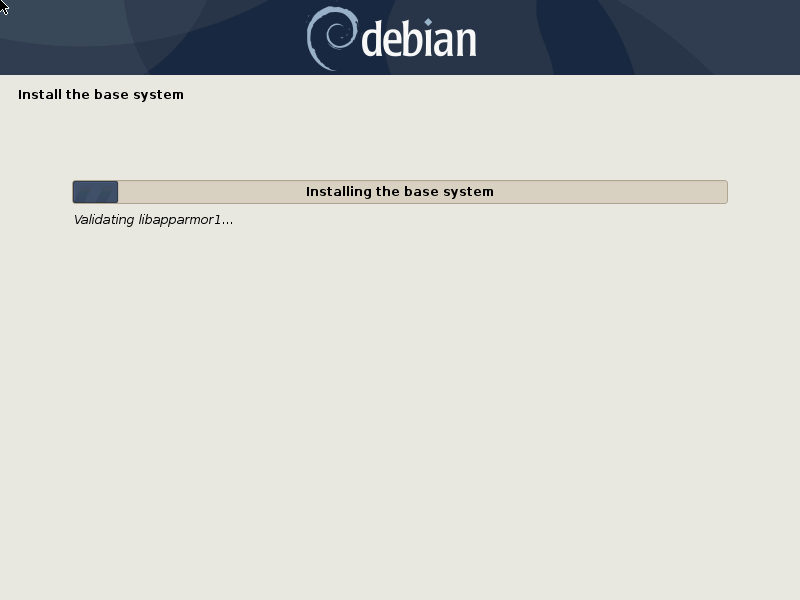
\includegraphics[width=.8\textwidth]{install}
    \caption*{مرحله نصب اولیه~\cite{fig:deb:install}}
  \end{figure}
\end{frame}
\note{
  این مرحله هیچ تعامل خاصی با کاربر ندارد و صرفا چند ابزار مانند apt و dpkg برای مدیریت پکیج‌های دبین نصب می‌کند.
  همچنین چند ابزار ضروری برای بوت کردن سیستم و شروع محیط‌ گرافیکی مانند GRUB، \lr{Xorg server}.

  گراب یک بوت لودر است برای بوت کردن کرنل‌های مختلف نصب شده یا سیستم عامل‌های دیگر موجود بر روی حافظه دستگاه.
  xorg نیز مدیر محیط گرافیکی است و مانند این ابزار زیاد است.
}
\section{پیکربندی}
\subdivider{پیکربندی}
\begin{frame}{پیکربندی پکیج منیجر}
  پکیج‌منیجر‌ها نیازمند مخازن و منابعی هستند تا از آنها پکیج‌ها را فراخوانی کنند.
  در این مرحله این مخازن تنظیم می‌شوند.
  \pic[.7]{mirror}{انتخاب سرور مخزن~\cite{fig:deb:mirror}}
\end{frame}
\note{
  این بخش تا جایی که ممکن به صورت خودکار انجام می‌شود. از شما می‌پرسد که پکیج‌ها از روی ایمیج بر روی دیسک نصب شود یا از طریق شبکه و اینترنت.

  اگر درخواست نصب پکیج‌ها از طریق شبکه داده شود؛ از شما دو سوال می‌پرسد که اول انتخاب کشور سرورها است و دوم انتخاب mirror (میرور‌ها سرورهای عمومی هستند که آینه کاملی از سرور اصلی پکیج‌های دبین هستند) است.
}
\begin{frame}{انتخاب پکیج‌ها}
  در این مرحله به شما اجازه داده می‌شود تا با توجه هدفتان در استفاده از سیستم پکیج‌های مورد نظر را نصب کنید.
  \pic[.7]{packages}{انتخاب پکیج‌ها مورد نیاز~\cite{fig:deb:packages}}
\end{frame}
\note{
  بعضی از گزینه‌های مربوط به محیط‌های گرافیکی هستند و بعضی‌ها نیز مربوط به درایورهای سخت‌افزارها.
  بعضی دیگر هم در مراحل جلوتر با توجه به سخت افزار‌های موجود به صورت خودکار نصب می‌شوند.
}
\subsection{نصب دیگر نرم‌افزارها و بروزرسانی سیستم}

% TODO move to another slide about packages
% \begin{frame}{نصب دیگر نرم‌افزارها و بروزرسانی سیستم}
%   شما می‌توایند پکیج‌های مورد نیاز را به ازای هر کاربر نصب کنید، برای مدیریت پکیج‌ها و اتوماتیک کردن مراحل نصب می‌توانید از ابزارهای مدیریت پکیج استفاده کنید که شامل apt و synaptic می‌شوند که هر دو تحت محیط متنی هستند.
%   شما می‌توانید به طور دستی هر پکیجی که خواستید به وسیله apt نصب کنید یا آن را حذف کنید.
%   با کلمه کلید «install» می‌توایند پکیجی نصب کنید و یا با استفاده از «uninstall» می‌توانید پکیجی را حذف کنید.

%   برای به روز رسانی سیستم و پکیج‌ها از دستور «apt upgrade» استفاده می‌شود که به طور خودکار تمام پکیج‌های نصب شده بر روی سیستم را به روزرسانی می‌کند.
% \end{frame}

\refs
\end{document}
